\documentclass[journal,onecolumn]{IEEEtran}

\makeatletter
\def\endthebibliography{%
	\def\@noitemerr{\@latex@warning{Empty `thebibliography' environment}}%
	\endlist
}
\makeatother
\usepackage{hyperref}
\usepackage{listings}
\usepackage{color}


\usepackage[utf8]{inputenc}

% Default fixed font does not support bold face
\DeclareFixedFont{\ttb}{T1}{txtt}{bx}{n}{10} % for bold
\DeclareFixedFont{\ttm}{T1}{txtt}{m}{n}{10}  % for normal
\definecolor{deepblue}{rgb}{0,0,0.5}
\definecolor{deepred}{rgb}{0.6,0,0}
\definecolor{deepgreen}{rgb}{0,0.5,0}



% Python style for highlighting
\newcommand\pythonstyle{\lstset{
		language=Python,
		basicstyle=\ttm,
		morekeywords={self},              % Add keywords here
		keywordstyle=\ttb\color{deepblue},
		emph={MyClass,__init__},          % Custom highlighting
		emphstyle=\ttb\color{deepred},    % Custom highlighting style
		stringstyle=\color{deepgreen},
		frame=tb,                         % Any extra options here
		showstringspaces=false
}}

% Python environment
\lstnewenvironment{python}[1][]
{
	\pythonstyle
	\lstset{#1}
}
{}

\usepackage{graphicx}
\graphicspath{ {./Material/pictures/} }




% *** CITATION PACKAGES ***
%
%\usepackage{cite}
% cite.sty was written by Donald Arseneau
% V1.6 and later of IEEEtran pre-defines the format of the cite.sty package
% \cite{} output to follow that of the IEEE. Loading the cite package will
% result in citation numbers being automatically sorted and properly
% "compressed/ranged". e.g., [1], [9], [2], [7], [5], [6] without using
% cite.sty will become [1], [2], [5]--[7], [9] using cite.sty. cite.sty's
% \cite will automatically add leading space, if needed. Use cite.sty's
% noadjust option (cite.sty V3.8 and later) if you want to turn this off
% such as if a citation ever needs to be enclosed in parenthesis.
% cite.sty is already installed on most LaTeX systems. Be sure and use
% version 5.0 (2009-03-20) and later if using hyperref.sty.
% The latest version can be obtained at:
% http://www.ctan.org/pkg/cite
% The documentation is contained in the cite.sty file itself.
\hyphenation{op-tical net-works semi-conduc-tor}


\begin{document}
	%
	% paper title
	% Titles are generally capitalized except for words such as a, an, and, as,
	% at, but, by, for, in, nor, of, on, or, the, to and up, which are usually
	% not capitalized unless they are the first or last word of the title.
	% Linebreaks \\ can be used within to get better formatting as desired.
	% Do not put math or special symbols in the title.
	\title{Distance and Movement Measurement of an Object\\ based on Stereo Images}

	\author{Lennard~Rose,~5110000,~FHWS
		Moritz~Zeitler,~5118094,~FHWS% <-this % stops a space
	}
	% The paper headers
	\markboth{Seminar Smart Systems}%
	{Shell \MakeLowercase{\textit{et al.}}: Bare Demo of IEEEtran.cls for IEEE Journals}

	% make the title area
	\maketitle

	% As a general rule, do not put math, special symbols or citations
	% in the abstract or keywords.
	\begin{abstract}
		This paper explains how to compute distance to, and movement of an object within vision of a stereo camera.
		Included is the whole workflow consisting of all steps that have to be made to get such a recognition to work. These steps are the hardware setup, all calibration steps, object detection, object tracking and the measurements of the values themselves.
	\end{abstract}


	% For peer review papers, you can put extra information on the cover
	% page as needed:
	% \ifCLASSOPTIONpeerreview
	% \begin{center} \bfseries EDICS Category: 3-BBND \end{center}
	% \fi
	%
	% For peerreview papers, this IEEEtran command inserts a page break and
	% creates the second title. It will be ignored for other modes.
	\IEEEpeerreviewmaketitle

	\section{Introduction}
\label{sec:einfuehrung}
From a high level standpoint the human eye is a very simple complex. It enables us to see things, even in color. But if we go deeper there is much more to our sight. For example we can see depth, which is very complex as a concept. This is based on the human eye having to different point-of-views. In this project the so called Stereo-Vision, will be translated to a computational level. To establish this we use a stereo camera setup to take photos/videos, create a depth map and try to compute the distance and movement of an object. The following chapters will describe this in a step by step fashion, starting with the theory behind it and the implementation afterwards.

\section{Workflow}
This chapter contains a detailed theoretical and practical description of each individual step in the workflow.
\subsection{Stereo Camera Calibration}
Cameras are projecting a three dimensional object to a two dimensional image. This projection is never alone determined by the original object, but also by all parameters of the used camera. These you can separate in two groups, external and internal. External parameters are the camera orientation in different planes. Internal parameters are determined by the cameras internal characteristics.\newline
\begin{figure}[h!]
	\centering
	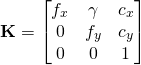
\includegraphics[scale=1]{intrinsicMatrix.png}
	\caption{Intrinsic Matrix}
\end{figure}
We can represent these internal parameters as an upper triangular matrix K. This matrix has the values fx and fy as the x and y focal lengths. cx and cy as the x and y coordinates of the optical center in the image plane. Gamma is the distortion between the axes, this value is replaced by a "0" in OpenCV´s calibration function.\newline
\begin{figure}[h!]
	\centering
	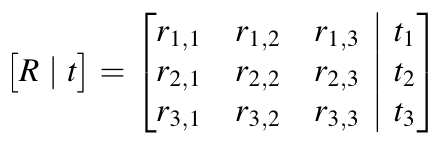
\includegraphics[scale=0.7]{extrinsicMatrix.png}
	\caption{Extrinsic Matrix}
\end{figure}
The external parameters are represented by an 3x3 rotation matrix, that indicates the rotation bias of the camera, combined with an 3x1 translation vector.\newline
\begin{figure}[h!]
	\centering
	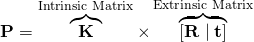
\includegraphics[scale=0.7]{projectionMatrix.png}
	\caption{Projection Matrix}
\end{figure}
Together these form the 3x4 Projection Matrix. This matrix and the 3D-coordinates of our point is used to calculate the image coordinates of the 2D projection. Calibration does nothing else than alter these matrices so our 2D projection matches the 3D object. This is usually done by giving the calibrating program/ function a set of 2D images with known 3D coordinates.\newline
This Calibration consists of two steps removing of Distortion as well as rectifying the images\cite{ImageRectification}.
\subsubsection{Distortion}
A camera lens always has some kind of curvature. This curvature is also visible in an image taken with this lens. This is called distortion. There are many different types of distortion which can be seen in the picture beneath.
\begin{figure}[h!]
	\centering
	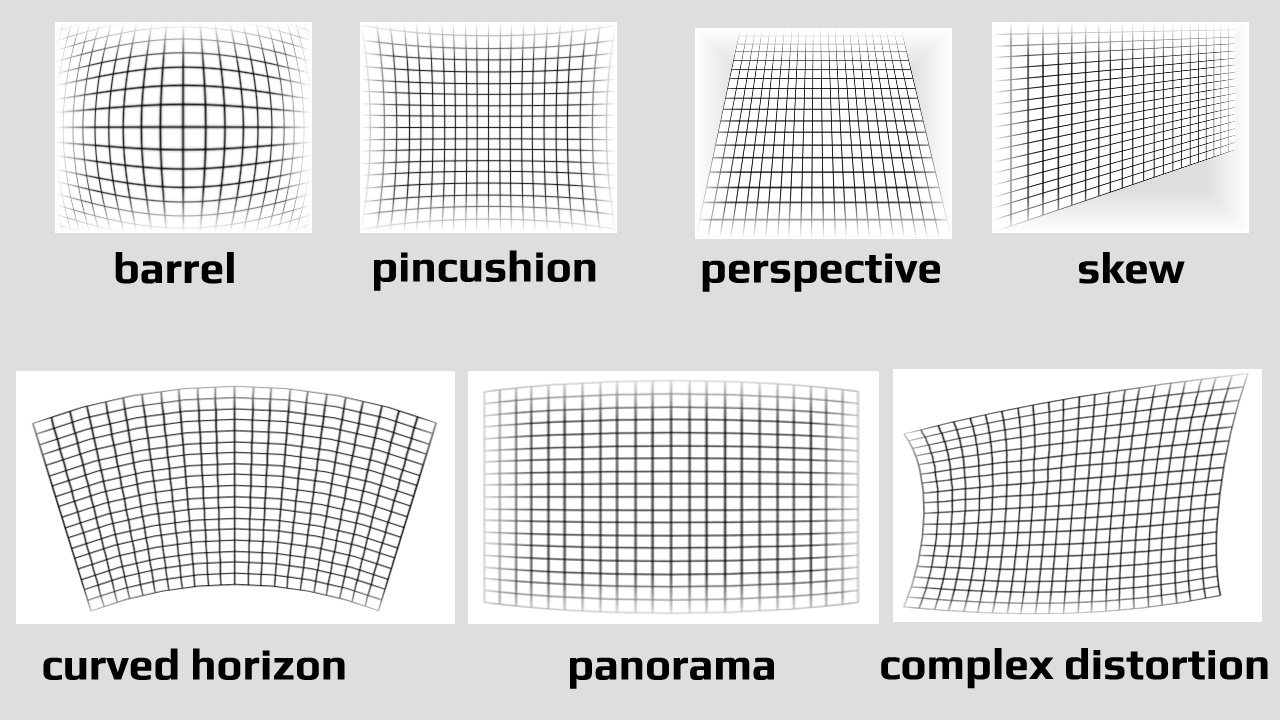
\includegraphics[scale=0.3]{distortion.jpg}
	\caption{Distortion types}
\end{figure}
To remove this distortion we take pictures of a chessboard. OpenCV, the package we use to do all calibration steps, can easily detect key points using this chessboard pattern. This is based on the big difference in pixel values between white and black. In combination with the size of the squares as well as the amount of the squares, OpenCV is able to create a calibration matrix removing the distortion.\newline
A very important part is to be very precise while taking the calibration pictures. To get a good result you need to take calibration photos, basically of all parts of the pov of the camera.\newline
The python implementation looks like the following:\\
First of all we convert the input picture to grayscale and feed it into a detection function for chessboard corners.
\begin{python}
	ret, corners = cv2.findCirclesGrid(inputImage,
	(chessboardColumns, chessboardRows),
	None)
\end{python}
As input we have the chessboard picture, columns of the chessboard, rows of the chessboard and an output array we don't use.
This function results in a return value whether a chessboard got detected and if so the 2D points of the chessboard corners. If the detection was successful the returned points get even more refined using:
\begin{python}
	cv2.cornerSubPix(inputImage,
	corners,
	(11, 11),
	(-1, -1),
	criteria)
\end{python}
The 'cornerSubPix' of openCV refines the corner locations \cite{forstner} of the checkboard.

\subsubsection{Rectification}
With image rectification, the goal is to project the two different images taken by the camera onto a common image plane. Through this process we make sure that the individual lines of
\subsection{Stereoscopy}
\subsection{Disparity Map}
\subsection{Depth Map}
\subsection{Object Detection}
\subsection{Object Tracking}
\subsection{Measurements}
\subsubsection{Distance}
\subsection{Direction}
\subsection{Speed}
\section{Prerequisites}
\section{Results}
\section{Conclusion}

\appendices

% can use a bibliography generated by BibTeX as a .bbl file
% BibTeX documentation can be easily obtained at:
% http://mirror.ctan.org/biblio/bibtex/contrib/doc/
% The IEEEtran BibTeX style support page is at:
% http://www.michaelshell.org/tex/ieeetran/bibtex/
%\bibliographystyle{IEEEtran}
% argument is your BibTeX string definitions and bibliography database(s)
\bibliography{bibtex/bib/IEEEabrv.bib,bibtex/bib/IEEEexample.bib}{}
\bibliographystyle{IEEEtran}

%
% <OR> manually copy in the resultant .bbl file
% set second argument of \begin to the number of references
% (used to reserve space for the reference number labels box)

\end{document}